\chapter{Preliminaries}
\label{ch:preliminaries}

\todo[inline]{fluff text}

\section{Graph Theory}
\label{sec:graphtheory}

Road networks can be modeled as graphs.
A graph \(G\) is formally defined as a pair \((V, E)\), where \(V\) represents a finite set of vertices (or nodes) and \(E\) represents a set of edges connecting pairs of vertices.
In many applications, particularly route planning, graphs are augmented with a weight function \(w: E \to \mathbb{R}^+\), assigning a positive real value such as distance or travel time to each edge.
However, for the purpose of this thesis, the topological strucuture of the graph is of primary interest, and we will not focus on edge weights.
We will also only consider simple graphs, meaning graphs without multiple edges between the same pair of vertices and without edges connecting a vertex to itself (loops).
Furthermore, as the concept of separators primarily applies to connectivity, we will consider undirected graphs, where edges represent symmetric relationships.
An edge connecting vertices \(u\) and \(v\) in an undirected graph is denoted as the set \(\{u,v\}\).
The neighborhood of a vertex \(v\) is defined as the set of vertices adjacent to \(v\), denoted as \(N : V \to \mathcal{P}(V)\).

A graph \emph{embedding} assigns each vertex \(v \in V\) of a graph \(G = (V, E)\) to a unique point \(p\) in a specific geometric space, such as the Euclidean plane \(\mathbb{R}^2\) or the surface of a sphere, where edges are represented as straight line segments connecting the points corresponding to their incident vertices.

\section{Graph Separators}
\label{sec:graphseparators}

A vertex separator (or simply separator) of a graph \(G = (V, E)\) is a subset of vertices \(S \subseteq V\) whose removal disconnects the graph into two or more components.
More formally, the subgraph induced by \(V \setminus S\), denoted \(G[V \setminus S]\), is disconnected.
For algorithmic applications, particularly divide-and-conquer strategies, balanced separators are crucial.

Let \(V_1, \dots, V_k\) be the vertex sets corresponding to the connected components of the subgraph \(G[V \setminus S]\).
Most often, the removal of such a separator yields exactly two components (\(k=2\)), as partitioning the graph into a larger number of components generally demands a larger separator.
For a given constant \(\alpha \in (0, 1)\), a separator \(S\) is termed \(\alpha\)-balanced if the size of every resulting component \(V_i\) is bounded.
Specifically, the condition \(|V_i| \leq \alpha |V|\) must hold for all \(i \in \{1, \dots, k\}\).
A simple illustration of a balanced separator is shown in \cref{fig:separator_example_balanced}.
A common requirement is \(2/3\)-balancedness, meaning each component contains at most \(2/3\) of the original graph's vertices.
Balancedness ensures that recursive applications of the separator lead to subproblems of substantially smaller size, which is essential for the efficiency of algorithms based on this technique.

Furthermore, minimizing the size of the separator \(S\) itself is critical for algorithmic performance.
The size of the separator is typically evaluated asymptotically as a function of the number of vertices \(n = |V|\) e.g. \(n^\beta\) for \(\beta \in (0,1)\).

The concept of \emph{recursive} \(\alpha\)-balanced separators extends this idea by ensuring that the property of finding small, balanced separators persists in the resulting subgraphs.
Specifically, after removing an \(\alpha\)-balanced separator \(S\) from \(G\), each induced subgraph \(G[V_i]\) (for \(i = 1, 2, \dots, k\)) can itself be partitioned using another \(\alpha\)-balanced separator of small size.

\begin{figure}
	\centering
	\begin{subfigure}{0.45\linewidth}
		\centering
		\begin{tikzpicture}[every node/.style={circle, draw, minimum size=0.7cm}]
			\node (1) {1};
			\node (2) [right=of 1] {2};
			\node (3) [right=of 2] {3};
			\node (4) [below=of 1] {4};
			\node (5) [below=of 2, fill=teal!30] {5};
			\node (6) [below=of 3] {6};
			\node (7) [below=of 4] {7};
			\node (8) [below=of 5, fill=teal!30] {8};

			\draw (4) -- (5);
			\draw (5) -- (7);
			\draw (5) -- (2);
			\draw (6) -- (5);
			\draw (7) -- (8);
			\draw (8) -- (6);
			\draw (4) -- (1);
			\draw (7) -- (4);
			\draw (2) -- (3);
			\draw (3) -- (6);
		\end{tikzpicture}
		\caption{\(G\) with separator \(S = \{5, 8\}\)}
	\end{subfigure}
	\hfill
	\begin{subfigure}{0.45\linewidth}
		\centering
		\begin{tikzpicture}[every node/.style={circle, draw, minimum size=0.7cm}]
			\node (1) {1};
			\node (2) [right=of 1] {2};
			\node (3) [right=of 2] {3};
			\node (4) [below=of 1] {4};
			\node (6) [below=of 3] {6};
			\node (7) [below=of 4] {7};

			\draw (4) -- (1);
			\draw (7) -- (4);
			\draw (2) -- (3);
			\draw (3) -- (6);
		\end{tikzpicture}
		\caption{\(G[V \setminus S]\)}
	\end{subfigure}
	\caption{Example of a well balanced separator in a graph. The vertices 5 and 8 form a balanced separator that disconnects the graph into two components.}
	\label{fig:separator_example_balanced}
\end{figure}

To compute separators, various algorithms can be employed.
In this thesis, we primarily utilize InertialFlowCutter \cite{gottesburen_faster_2019}.
This algorithm leverages geometric embeddings, often available for road networks, to compute high-quality node orderings efficiently.
These node orderings serve as the basis for extracting separators from the graph using the method described below.
However, InertialFlowCutter requires such a geometric embedding as input.
In cases where a geometric embedding was not available for a graph, we utilized the KaHIP (Karlsruhe High Quality Partitioning) framework \cite{sanders_think_2013}.
Although known for graph partitioning, KaHIP includes algorithms for computing separators directly.

When using InertialFlowCutter, the resulting node ordering is interpreted as an elimination order for the vertices of the graph \( G = (V, E) \).
Based on this order, a chordal supergraph \( G' = (V, E \cup F) \) is implicitly constructed, where \( F \) represents the fill-in edges.
This process can be visualized by processing vertices in reverse elimination order.
For each vertex \(v\), edges are added to make its neighbors that appear later in the order form a clique.
An efficient way to implement this chordalization involves connecting, for each node \(v\) (in reverse order), all its higher-numbered neighbors to its lowest-numbered neighbor among them.

Simultaneously, a tree structure \(T\) based on this ordering can be constructed.
Each node \(v \in V\) selects its parent in the tree as the neighbor \(u\) that appears earliest in the elimination order among all neighbors \(w\) with \( \text{rank}(w) > \text{rank}(v) \).
If a node has no neighbors later in the order, it becomes the root.

Separators in the original graph \(G\) can be derived from this tree structure using a traversal algorithm.
The fundamental idea is to identify paths representing non-branching segments of the tree.
Starting from a node \(r\) (representing the current subgraph), the traversal follows a path \(P = (v_1=r, v_2, \dots, v_k)\) downwards, where each node \(v_i\) (\(1 \le i < k\)) has exactly one child \(v_{i+1}\) in the tree.
The path ends at node \(v_k\), which is the first node encountered that does not have exactly one child (i.e., it has zero or multiple children).
The set of vertices on this path, \(S = \{v_1, v_2, \dots, v_k\}\), forms a potential separator.
Its size is \(k\), the number of nodes on the path.
The traversal algorithm continues recursively into these subtrees.
An overview of this process is illustrated in \cref{fig:extract_separator_from_order}.

For practical application in this thesis, particularly to ensure balanced partitions, this core logic is refined by introducing a significance threshold based on subtree sizes.
This threshold defines whether a child node represents a sufficiently large part of the graph to be considered relevant for partitioning (e.g., exceeding a fraction of the parent's subtree size).
In the refined process, the traversal path \(P\) only extends from \(v_i\) to \(v_{i+1}\) if \(v_{i+1}\) is the single child of \(v_i\) that meets this significance threshold.
A node \(v_k\) is identified as a branching point yielding a separator \(S = \{v_1, \dots, v_k\}\) only if it has two or more children meeting the threshold.

\begin{figure}
	\begin{subfigure}{0.3\textwidth}
		\centering
		\begin{tikzpicture}[every node/.style={circle, draw, minimum size=0.7cm}]
			\node (4) {4};
			\node (1) [right=of 4] {1};
			\node (2) [below=of 4] {2};
			\node (3) [right=of 2] {3};

			\draw (4) -- (1) -- (3) -- (2) -- (4);
		\end{tikzpicture}
		\caption{Original graph \(G\)\newline}
	\end{subfigure}
	\hfill
	\begin{subfigure}{0.3\textwidth}
		\centering
		\begin{tikzpicture}[every node/.style={circle, draw, minimum size=0.7cm}]
			\node (4) {4};
			\node (1) [right=of 4] {1};
			\node (2) [below=of 4] {2};
			\node (3) [right=of 2] {3};

			\draw (4) -- (1) -- (3) -- (2) -- (4);
			\draw[dashed] (4) -- (3);
		\end{tikzpicture}
		\caption{Chordal supergraph based on the order}
	\end{subfigure}
	\hfill
	\begin{subfigure}{0.3\textwidth}
		\centering
		\begin{tikzpicture}[every node/.style={circle, draw, minimum size=0.7cm, distance=0.1cm}, node distance=0.5cm and 0.8cm]
			\node (3) [fill=teal!30]{3};
			\node (4) [above=of 3, fill=teal!30] {4};
			\node (1) [below left=of 3] {1};
			\node (2) [below right=of 3] {2};

			\draw (3) -- (1);
			\draw (3) -- (2);
			\draw (3) -- (4);
		\end{tikzpicture}
		\caption{Derived tree \(T\), Separator \{4,3\} highlighted}
	\end{subfigure}
	\caption{Example Process of deriving a separator from a node order. Node labels in indicate their rank in the node order.}
	\label{fig:extract_separator_from_order}
\end{figure}

\section{Customizable Contraction Hierarchies}
\label{sec:cch}

Efficiently computing shortest paths in large graphs, such as continental road networks, is a fundamental problem.
While Dijkstra's algorithm provides exact solutions for single-source shortest paths, its performance can be insufficient for real-time applications on large datasets.
For instance, executing Dijkstra's algorithm on a graph representing the European road network can take over a second.
To accelerate query performance, many algorithms employ a two-phase approach: an initial precomputation phase followed by a query phase.
This precomputation step processes the graph structure and edge weights to generate auxiliary data structures that enable faster subsequent queries.

However, edge weights in real-world networks, particularly road networks, are often dynamic due to factors like traffic congestion.
Standard two-phase approaches typically require re-running the entire, often time-consuming, precomputation phase whenever edge weights change.
To address this limitation, three-phase approaches have been developed \cite{delling_customizable_2011}, separating the process into precomputation, customization, and query phases.
The initial precomputation relies only on the graph's topology (nodes and edges), which is assumed to be relatively static.
The second phase, customization, quickly incorporates the current edge weights into the precomputed structures.
Finally, the query phase uses the customized data structures to answer shortest path requests rapidly.

Customizable Contraction Hierarchies (CCH) represent a prominent and effective three-phase route planning technique \cite{dibbelt_customizable_2016}.
CCH enables fast customization, allowing adaptation to frequently changing edge weights, making it suitable for dynamic scenarios.
The core idea underpinning CCH involves strategically inserting shortcut edges into the graph, analogous to the concept used in the original Contraction Hierarchies (CH) algorithm \cite{geisberger_contraction_2008}.
These shortcuts bypass sequences of original edges, effectively contracting the graph and speeding up queries.
The efficiency of the CCH precomputation, particularly the node ordering it employs, can leverage the existence of small separators.
We will now give a quick overview of the CCH algorithm.

\paragraph{Precomputation}

The CCH precomputation phase introduces shortcut edges based on a given vertex order.
These shortcuts effectively bypass sections of the graph, allowing algorithms to skip over entire subgraphs, unless the target node resides within such a subgraph.
Furthermore, the specific process of inserting shortcuts based on the contraction order guarantees that any shortest path in the original graph corresponds to an 'up-down' path in the hierarchy defined by the vertex ranks \cite{geisberger_contraction_2008}.
An 'up-down' path consists of a sequence of edges leading to vertices with increasing ranks (the 'up' segment), followed by a sequence of edges leading to vertices with decreasing ranks (the 'down' segment).
This property enables efficient bidirectional search by restricting exploration to higher-ranked neighbors.

This order is defined by a bijection \( \pi : \{1, \dots, n\} \to V \), where \( n = |V| \).
We will call the inverse of this order \( \text{rank} : V \to \{1, \dots, n\} \), which assigns each vertex its position in the order.
The core process involves iteratively contracting vertices in order of their rank, starting from rank 1 up to \( n \).
Contracting a vertex \( v_i \) involves removing it and its incident edges from the current graph representation.
For every pair of (higher ranked) neighbors \( u, w \in N(v_i) \), a shortcut edge \( (u, w) \) is introduced.
Resulting multi-edges are simplified.
We call the resulting graph \( G_C = (V, E_C) \), where \( E_C = E \cup F \) and \( F \) represents the set of shortcut edges.
The contraction process is illustrated in \cref{fig:cch_precomputation_example}.

\begin{figure}
	\begin{subfigure}{0.45\linewidth}
		\centering
		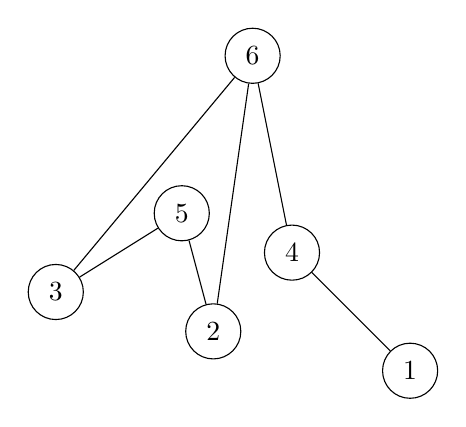
\begin{tikzpicture}[every node/.style={circle, draw, minimum size=0.7cm}]
			\node (3) at (-0.5,2) {3};
			\node (5) at (1.1,3) {5};
			\node (2) at (1.5,1.5) {2};
			\node (6) at (2,5) {6};
			\node (4) at (2.5,2.5) {4};
			\node (1) at (4,1) {1};

			\draw (3) -- (6);
			\draw (3) -- (5);
			\draw (5) -- (2);
			\draw (2) -- (6);
			\draw (1) -- (4);
			\draw (4) -- (6);
		\end{tikzpicture}
		\caption{Input graph. Already converted to be undirected and simple.}
	\end{subfigure}
	\hfill
	\begin{subfigure}{0.45\linewidth}
		\centering
		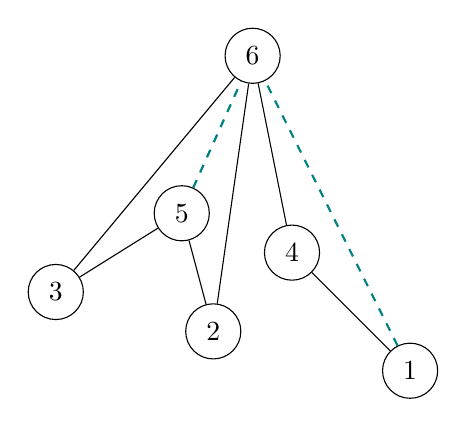
\begin{tikzpicture}[every node/.style={circle, draw, minimum size=0.7cm}]
			\node (3) at (-0.5,2) {3};
			\node (5) at (1.1,3) {5};
			\node (2) at (1.5,1.5) {2};
			\node (6) at (2,5) {6};
			\node (4) at (2.5,2.5) {4};
			\node (1) at (4,1) {1};

			\draw (3) -- (6);
			\draw (3) -- (5);
			\draw (5) -- (2);
			\draw (2) -- (6);
			\draw (1) -- (4);
			\draw (4) -- (6);

			\draw[thick, teal, dashed] (5) -- (6);
			\draw[thick, teal, dashed] (1) -- (6);
		\end{tikzpicture}
		\caption{Graph after precomputation, new shortcut edges are shown in teal.}
	\end{subfigure}
	\caption{Example of the CCH precomputation step. Nodes are named and positioned based on their rank.}
	\label{fig:cch_precomputation_example}
\end{figure}

A primary objective when selecting the vertex order is to minimize the number of shortcut edges introduced during the contraction process.
Minimizing shortcuts is beneficial for both storage and query efficiency \cite{dibbelt_customizable_2016}.
However, solely minimizing the number of added shortcuts may not be sufficient in all cases.
Different heuristics for selecting the contraction order exist.

\paragraph{Nested Dissection}

One method for computing good vertex orders are Nested Dissections.
The process begins by identifying a small, balanced separator in the graph.
Nodes within this separator are conceptually removed, partitioning the graph into smaller components.
These separator nodes are designated as high-rank nodes in the hierarchy and are consequently placed towards the end of the final node ordering.
This procedure is then applied recursively to the remaining components.
\Cref{fig:nested_dissection_example} provides a visual representation of this recursive partitioning strategy.

\begin{figure}
	\centering
	\begin{tikzpicture}[every node/.style={circle, draw, minimum size=1cm}]
		\node (10)                {1};
		\node (20)  [right=of 10, fill=purple!30] {3};
		\node (30)  [right=of 20] {2};
		\node (40)  [right=of 30, fill=teal!30] {21};
		\node (50)  [right=of 40] {11};
		\node (60)  [right=of 50, fill=orange!30] {18};
		\node (70)  [right=of 60] {14};

		\node (11)  [below=of 10, fill=orange!30] {9};
		\node (21)  [below=of 20, fill=orange!30] {8};
		\node (31)  [below=of 30, fill=orange!30] {7};
		\node (41)  [below=of 40, fill=teal!30] {20};
		\node (51)  [below=of 50, fill=purple!30] {12};
		\node (61)  [below=of 60, fill=orange!30] {17};
		\node (71)  [below=of 70, fill=purple!30] {15};

		\node (12)  [below=of 11] {4};
		\node (22)  [below=of 21, fill=purple!30] {6};
		\node (32)  [below=of 31] {5};
		\node (42)  [below=of 41, fill=teal!30] {19};
		\node (52)  [below=of 51] {10};
		\node (62)  [below=of 61, fill=orange!30] {16};
		\node (72)  [below=of 71] {13};

		\draw (10) -- (20) -- (30) -- (40) -- (50) -- (60) -- (70);
		\draw (11) -- (21) -- (31) -- (41) -- (51) -- (61) -- (71);
		\draw (12) -- (22) -- (32) -- (42) -- (52) -- (62) -- (72);
		\foreach \i in {1,...,7} { \draw (\i0) -- (\i1) -- (\i2); }
	\end{tikzpicture}
	\caption{Example of a Nested Dissection. The top level separator is shown in teal, the second level in orange and the third level in purple. The nodes are named according to their rank in the resulting order.}
	\label{fig:nested_dissection_example}
\end{figure}

\paragraph{Customization}

Customization assigns the current metric's weights to the original edges within the CCH supergraph \(G_C\) and initializes shortcut edge weights to infinity. Following this initialization, edge weights are systematically updated to ensure the triangle inequality holds throughout \(G_C\).

To achieve this, the concept of a lower triangle is employed.
Given an edge \(\{x, y\} \in E_C\), a lower triangle is formed by the vertices \(\{x, y, z\}\) if the edges \(\{z, x\}\) and \(\{z, y\}\) also exist, and \(rank(z) < \min\{rank(x), rank(y)\}\).
The customization algorithm iterates through the vertices of the graph in ascending order of their precomputed rank.
For each vertex \(x\), it considers all upward edges \(\{x, y\}\) in the graph, where \(y\) is a neighbor of \(x\) and \(rank(y) > rank(x)\).
For every such edge \(\{x, y\}\) we determine all lower triangles \(\{x, y, z\}\).
If the path through \(z\) offers a shorter connection, the weight of the edge \(\{x, y\}\) is updated to this smaller value: \(w(x, y) \leftarrow \min\{w(x, y), w(x, z) + w(z, y)\}\).
The detailed procedure is outlined in the pseudocode presented in \cref{alg:customization}.
An illustration of the customization process is provided in \cref{fig:cch_precomputation_example}.

Note that the outlined algorithm only considers undirected edge weights, the algorithm can be extendend to directed edge weights. Details can be found in \cite{dibbelt_customizable_2016}.

\begin{algorithm}
	\Input{\( G_C = (V, E_C) \), node ordering \(\pi\), edge weights \(w\)}
	\Output{Customized CCH graph}
	\BlankLine
	\ForAll{\(x\) in \(V\) in ascending order of rank}{
		\ForAll{upward edges \( \{x, y\} \) in \( E_C \)}{
			\ForAll{lower triangles \( \{x, y, z\} \) associated with \( \{x, y\} \)}{
				\( w(x, y) \longleftarrow \min\{ w(x, y), w(x, z) + w(z, y) \} \)\;
			}
		}
	}
	\caption{CCH Customization}
	\label{alg:customization}
\end{algorithm}

\begin{figure}
	\begin{subfigure}{0.45\linewidth}
		\centering
		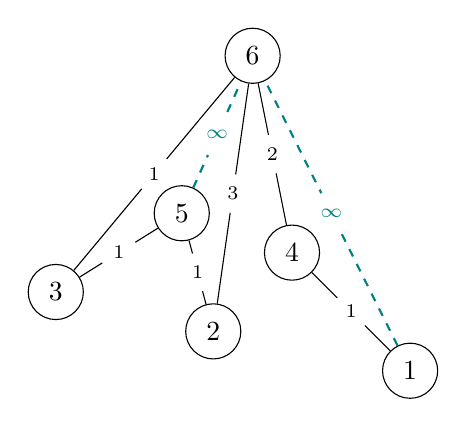
\begin{tikzpicture}
			\begin{scope}[every node/.style={circle, draw, minimum size=0.7cm}]
				\node (3) at (-0.5,2) {3};
				\node (5) at (1.1,3) {5};
				\node (2) at (1.5,1.5) {2};
				\node (6) at (2,5) {6};
				\node (4) at (2.5,2.5) {4};
				\node (1) at (4,1) {1};
			\end{scope}

			\begin{scope}[every node/.style={midway, fill=white, font=\scriptsize, inner sep=1mm, circle}]
				\draw (3) -- (6) node {1};
				\draw (3) -- (5) node {1};
				\draw (2) -- (5) node {1};
				\draw (2) -- (6) node {3};
				\draw (1) -- (4) node {1};
				\draw (4) -- (6) node {2};
				\draw[thick, teal, dashed] (5) -- (6) node {\(\infty\)};
				\draw[thick, teal, dashed] (1) -- (6) node {\(\infty\)};
			\end{scope}
		\end{tikzpicture}
		\caption{Graph after precomputation. Weights are added to the edges. Shortcuts get weight \(\infty\).}
	\end{subfigure}
	\hfill
	\begin{subfigure}{0.45\linewidth}
		\centering
		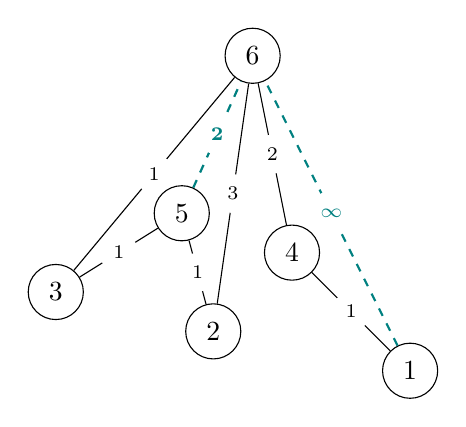
\begin{tikzpicture}
			\begin{scope}[every node/.style={circle, draw, minimum size=0.7cm}]
				\node (3) at (-0.5,2) {3};
				\node (5) at (1.1,3) {5};
				\node (2) at (1.5,1.5) {2};
				\node (6) at (2,5) {6};
				\node (4) at (2.5,2.5) {4};
				\node (1) at (4,1) {1};
			\end{scope}

			\begin{scope}[every node/.style={midway, fill=white, font=\scriptsize, inner sep=1mm, circle}]
				\draw (3) -- (6) node {1};
				\draw (3) -- (5) node {1};
				\draw (2) -- (5) node {1};
				\draw (2) -- (6) node {3};
				\draw (1) -- (4) node {1};
				\draw (4) -- (6) node {2};
				\draw[thick, teal, dashed] (5) -- (6) node {\textbf{2}};
				\draw[thick, teal, dashed] (1) -- (6) node {\(\infty\)};
			\end{scope}
		\end{tikzpicture}
		\caption{Graph after customization. The shortcut edge \(\{5, 6\}\) is updated to weight \(2\).}
	\end{subfigure}
	\caption{Example of the CCH customization step.}
\end{figure}

\paragraph{Query}

To answer a shortest path query between a source node \(s\) and a target node \(t\), the algorithm utilizes an structure known as the elimination tree.
The elimination tree is defined on the nodes of \(G_C\).
The parent of a node \(v\) in the elimination tree is the neighbor \(p\) of \(v\) in the CCH graph that has the lowest rank among all neighbors with a rank strictly greater than the rank of \(v\).
\cref{fig:cch_elimination_tree} illustrates the elimination tree for the example graph shown in \cref{fig:cch_precomputation_example}.
The query algorithm performs a bidirectional search upwards in this elimination tree, starting from \(s\) and \(t\).

\begin{figure}
	\centering
	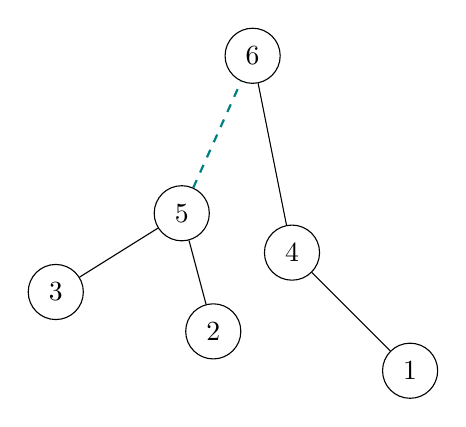
\begin{tikzpicture}[every node/.style={circle, draw, minimum size=0.7cm}]
		\node (3) at (-0.5,2) {3};
		\node (5) at (1.1,3) {5};
		\node (2) at (1.5,1.5) {2};
		\node (6) at (2,5) {6};
		\node (4) at (2.5,2.5) {4};
		\node (1) at (4,1) {1};

		\draw (3) -- (5);
		\draw (5) -- (2);
		\draw (1) -- (4);
		\draw (4) -- (6);

		\draw[thick, teal, dashed] (5) -- (6);
	\end{tikzpicture}
	\caption{Elimination tree for the example graph in \cref{fig:cch_precomputation_example}.}
	\label{fig:cch_elimination_tree}
\end{figure}

The core query process operates iteratively.
Let \(u_s\) and \(u_t\) be the current nodes in the upward search originating from \(s\) and \(t\), respectively; initially, \(u_s = s\) and \(u_t = t\).
The algorithm proceeds until the root of the elimination tree is reached.
In each step, the ranks of the current nodes \(u_s\) and \(u_t\) are compared.
If \(u_s\) has a smaller rank than \(u_t\), the algorithm relaxes all outgoing edges \(\{u_s, v_i\}\) present in \(G_C\).
Subsequently, \(u_s\) is updated to become its parent node in the elimination tree.
Otherwise (if \(u_t\) has a rank less than or equal to that of \(u_s\)), the algorithm relaxes all outgoing edges \(\{u_t, v_i\}\) existing in the CCH graph.
Following the relaxation step, \(u_t\) is updated to its parent in the elimination tree.
This process continues, effectively exploring paths upwards towards higher-ranked nodes.
The correctness of this query algorithm for computing shortest path distances has been established; a detailed proof, which is beyond the scope of this thesis, can be found in \cite{dibbelt_customizable_2016}.

\paragraph{Complexity}

The size of the separators found significantly impacts the efficiency of CCH queries.
CCH queries restrict exploration to edges leading towards higher-ranked nodes (upward edges).
Consider the separator identified at the highest level of the recursion, which contains approximately \(n^\beta\) nodes.
When a query initiates within a component defined by this separator, nodes located in other components cannot be reached without traversing downwards through a separator node, violating the upward search constraint.
This containment effect applies recursively within the sub-components generated during the nested dissection.
Let \( \alpha \) denote the balance factor.
The sub-components at recursion level \( i \) consequently have size at most \( \alpha^i \cdot n \).
Analyzing the total bound of the search space involves summing these separator sizes across the finite levels \(i\) of the recursion.
This sum can be bounded by approximating it with the corresponding infinite geometric series \cite{bauer_search-space_2016}:

\begin{align*}
	    & ~\sum_{i=0}^{\infty} (\alpha^i\cdot n)^\beta                                                         \\
	=   & ~n^\beta \cdot \sum_{i=0}^{\infty} \alpha^{i\cdot \beta}                                             \\
	=   & ~n^\beta \cdot \frac{1}{1 - \alpha^\beta} \qquad \text{Geometric series, since \(\alpha \in (0,1)\)} \\
	\in & ~\bigO{n^\beta}
\end{align*}

This analysis demonstrates that the total search space size explored during a CCH query is bounded by \(\bigO{n^\beta}\), under the assumption that small separators can be found recursively.
Note that we do not have worst case guarantees for the size of the separators in real road networks, but we can expect them to be small in practice.
Thus, the performance of the CCH algorithm is directly linked to the ability to find small separators.
